%Version 3.1 December 2024
% See section 11 of the User Manual for version history
%%%%%%%%%%%%%%%%%%%%%%%%%%%%%%%%%%%%%%%%%%%%%%%%%%%%%%%%%%%%%%%%%%%%%%
%%                                                                 %%
%% Please do not use \input{...} to include other tex files.       %%
%% Submit your LaTeX manuscript as one .tex document.              %%
%%                                                                 %%
%% All additional figures and files should be attached             %%
%% separately and not embedded in the \TeX\ document itself.       %%
%%                                                                 %%
%%%%%%%%%%%%%%%%%%%%%%%%%%%%%%%%%%%%%%%%%%%%%%%%%%%%%%%%%%%%%%%%%%%%%

%%\documentclass[referee,sn-basic]{sn-jnl}% referee option is meant for double line spacing

%%=======================================================%%
%% to print line numbers in the margin use lineno option %%
%%=======================================================%%

%%\documentclass[lineno,pdflatex,sn-basic]{sn-jnl}% Basic Springer Nature Reference Style/Chemistry Reference Style

%%=========================================================================================%%
%% the documentclass is set to pdflatex as default. You can delete it if not appropriate.  %%
%%=========================================================================================%%

%%\documentclass[sn-basic]{sn-jnl}% Basic Springer Nature Reference Style/Chemistry Reference Style

%%Note: the following reference styles support Namedate and Numbered referencing. By default the style follows the most common style. To switch between the options you can add or remove �Numbered� in the optional parenthesis.
%%The option is available for: sn-basic.bst, sn-chicago.bst%

\documentclass[pdflatex,sn-nature]{sn-jnl}% Style for submissions to Nature Portfolio journals
%\documentclass[pdflatex,sn-basic]{sn-jnl}% Basic Springer Nature Reference Style/Chemistry Reference Style
%\documentclass[pdflatex,sn-mathphys-num]{sn-jnl}% Math and Physical Sciences Numbered Reference Style
%\documentclass[pdflatex,sn-mathphys-ay]{sn-jnl}% Math and Physical Sciences Author Year Reference Style
%\documentclass[pdflatex,sn-aps]{sn-jnl}% American Physical Society (APS) Reference Style
%\documentclass[pdflatex,sn-vancouver-num]{sn-jnl}% Vancouver Numbered Reference Style
%\documentclass[pdflatex,sn-vancouver-ay]{sn-jnl}% Vancouver Author Year Reference Style
%\documentclass[pdflatex,sn-apa]{sn-jnl}% APA Reference Style
%\documentclass[pdflatex,sn-chicago]{sn-jnl}% Chicago-based Humanities Reference Style

%%%% Standard Packages
%%<additional latex packages if required can be included here>

\usepackage{graphicx}%
\usepackage{multirow}%
\usepackage{amsmath,amssymb,amsfonts}%
\usepackage{amsthm}%
\usepackage{mathrsfs}%
\usepackage[title]{appendix}%
\usepackage{xcolor}%
\usepackage{textcomp}%
\usepackage{manyfoot}%
\usepackage{booktabs}%
\usepackage{algorithm}%
\usepackage{algorithmicx}%
\usepackage{algpseudocode}%
\usepackage{listings}%

\usepackage{standalone}
\usepackage{tikz}
\usepackage[dvipsnames]{xcolor}
\usepackage{geometry}

% Minted package for beautiful syntax highlighting
\usepackage{minted}
\usemintedstyle{borland}
\setminted{
  fontsize=\small,
  breaklines=true,
  autogobble,
  frame=single,
  framesep=2mm,
  linenos
}

% Use bash lexer for TSG code examples (since it handles # comments well)
\newminted{bash}{
  fontsize=\small,
  breaklines=true,
  autogobble,
  frame=single,
  framesep=2mm,
  linenos
}

\usetikzlibrary{shadows,shapes,arrows,positioning,fit,backgrounds,decorations.pathreplacing,calc}

\graphicspath{{../figures}}

\usepackage[acronym, automake, style=index, shortcuts]{glossaries-extra}
\setabbreviationstyle[acronym]{long-short}
% define glossaries
\makeglossaries

\newacronym{wga}{WGA}{Whole Genome Amplification}
\newacronym{mda}{MDA}{Multiple Displacement Amplification}
\newacronym{malbac}{MALBAC}{Multiple Annealing and Looping-based Amplification Cycles}
\newacronym{gpu}{GPU}{Graphics Processing Unit}
\newacronym{hpc}{HPC}{High Performance Computing}
\newacronym{sv}{SV}{Structural Variation}

\newacronym{ide}{IDE}{Integrated Development Environment}
\newacronym{cd}{CD}{Continuous Development}
\newacronym{ucsc}{UCSC}{UCSC Genome Browser}
\newacronym{glm}{GLM}{Genomic Language Model}
\newacronym{lcglm}{LCGLM}{long-context genomic language model}
\newacronym{snp}{SNP}{Single Nucleotide Polymorphism}

\newacronym{mlp}{MLP}{multilayer perceptron}
\newacronym{ont}{ONT}{Oxford Nanopore Technologies}
\newacronym{pb}{PacBio}{Pacific Biosciences}

\newacronym{tsg}{TSG}{Transcriptome Segment Graph}
\newacronym{nlt}{NLT}{Non-colinear Transcript}

\newacronym{go}{GO}{Gene Ontology}
\newacronym{pcr}{PCR}{Polymerase Chain Reaction}
\newacronym{mrna}{mRNA}{messenger RNA}

%%%%%=============================================================================%%%%
%%%%  Remarks: This template is provided to aid authors with the preparation
%%%%  of original research articles intended for submission to journals published
%%%%  by Springer Nature. The guidance has been prepared in partnership with
%%%%  production teams to conform to Springer Nature technical requirements.
%%%%  Editorial and presentation requirements differ among journal portfolios and
%%%%  research disciplines. You may find sections in this template are irrelevant
%%%%  to your work and are empowered to omit any such section if allowed by the
%%%%  journal you intend to submit to. The submission guidelines and policies
%%%%  of the journal take precedence. A detailed User Manual is available in the
%%%%  template package for technical guidance.
%%%%%=============================================================================%%%%

%% as per the requirement new theorem styles can be included as shown below
\theoremstyle{thmstyleone}%
\newtheorem{theorem}{Theorem}%  meant for continuous numbers
%%\newtheorem{theorem}{Theorem}[section]% meant for sectionwise numbers
%% optional argument [theorem] produces theorem numbering sequence instead of independent numbers for Proposition
\newtheorem{proposition}[theorem]{Proposition}%
%%\newtheorem{proposition}{Proposition}% to get separate numbers for theorem and proposition etc.

\theoremstyle{thmstyletwo}%
\newtheorem{example}{Example}%
\newtheorem{remark}{Remark}%

\theoremstyle{thmstylethree}%
\newtheorem{definition}{Definition}%

\raggedbottom
%%\unnumbered% uncomment this for unnumbered level heads

\begin{document}

\title[Article Title]{ChimeraLM: A genomic language model for detecting whole genome amplification artifacts in single-cell sequencing}

%%=============================================================%%
%% GivenName	-> \fnm{Joergen W.}
%% Particle	-> \spfx{van der} -> surname prefix
%% FamilyName	-> \sur{Ploeg}
%% Suffix	-> \sfx{IV}
%% \author*[1,2]{\fnm{Joergen W.} \spfx{van der} \sur{Ploeg}
%%  \sfx{IV}}\email{iauthor@gmail.com}
%%=============================================================%%
\author[1]{\fnm{Yangyang} \sur{Li}}\email{yangyang.li@northwestern.edu}
% \equalcont{These authors contributed equally to this work.}

\author[1]{\fnm{Qingxiang} \sur{Guo}}\email{qingxiang.guo@northwestern.edu}
\equalcont{These authors contributed equally to this work.}

% \author*[1,2]{\fnm{First} \sur{Author}}\email{iauthor@gmail.com}
% \author[1]{\fnm{Ting-You} \sur{Wang}}\email{tywang@northwestern.edu}
% \equalcont{These authors contributed equally to this work.}

% \author[1]{\fnm{Qingxiang} \sur{Guo}}\email{qingxiang.guo@northwestern.edu}
\author*[1,2]{\fnm{Rendong} \sur{Yang}}\email{rendong.yang@northwestern.edu}

\affil[1]{\orgdiv{Department of Urology}, \orgname{Northwestern University Feinberg School of Medicine}, \orgaddress{\street{303 E Superior St}, \city{Chicago}, \postcode{60611}, \state{IL}, \country{USA}}}
\affil[2]{\orgdiv{Robert H. Lurie Comprehensive Cancer Center}, \orgname{Northwestern University Feinberg School of Medicine}, \orgaddress{\street{675 N St Clair St}, \city{Chicago}, \postcode{60611}, \state{IL}, \country{USA}}}

\abstract{
	this is a abtract
}
\keywords{Whole Genomics Amplification, Genomic Language Model}

\maketitle

\section*{Main}\label{sec:main}

Single-cell genomics has revolutionized our understanding of cellular heterogeneity and development by enabling the characterization of individual cells rather than bulk populations~\cite{kalef2024single, sun2024mapping}.
This approach has proven instrumental in uncovering rare cell types, tracking developmental trajectories, and identifying somatic mutations that drive disease progression.
However, the limited amount of DNA present in a single cell, typically only a few picograms, poses significant technical challenges for comprehensive genomic analysis~\cite{leung2016highly, gawad2016single}.

To overcome this fundamental limitation, \gls{wga} has become an essential preprocessing step in single-cell genomic studies~\cite{zong2012genome, huang2015single}.
Various \gls{wga} techniques, including \gls{mda}, \gls{malbac}, and other emerging methods, can amplify the entire genome from a single cell by several orders of magnitude, generating sufficient DNA material for high-coverage sequencing~\cite{de2014quantitative, biezuner2021comparison,fu2015uniform, agyabeng2025evaluating}.
This amplification enables researchers to achieve the depth and breadth of coverage necessary for reliable variant calling, copy number analysis, and structural variation detection.

Despite its critical role in single-cell genomics, \gls{wga} introduces systematic artifacts that can significantly impact downstream analyses~\cite{lu2023chimera, lu2023exploration}.
Among the most problematic are chimeric sequences\textemdash artificial DNA constructs formed when DNA fragments from different genomic loci are erroneously joined during the amplification process~\cite{lu2023chimera, lu2023exploration, agyabeng2025evaluating}.
These chimeric artifacts can manifest as false-positive structural variations that do not exist in the original cell~\cite{lu2023chimera}.
The presence of such artifacts poses a substantial challenge for accurate \gls{sv} detection, potentially leading to misinterpretation of genomic rearrangements and their biological significance.

Current computational approaches for identifying \gls{wga}-induced artifacts rely primarily on coverage-based metrics and read-pair orientation patterns~\cite{kiguchi2021long, lu2023exploration}.
However, these methods often fail to distinguish between genuine structural variations and amplification artifacts, particularly when chimeric sequences exhibit complex rearrangement patterns or occur in repetitive genomic regions~\cite{kosugi2019comprehensive, mahmoud2019structural}.
The lack of robust artifact detection methods has limited the reliability of structural variant analysis in single-cell studies and hindered the full realization of single-cell genomics' potential.

To address these challenges, we developed ChimeraLM, a genomic language model specifically designed to detect chimeric artifacts introduced by whole genome amplification.
By leveraging deep learning approaches to capture sequence patterns and contextual information in genomic reads~\cite{dalla2025nucleotide, zhou2023dnabert, nguyen2023hyenadna}, ChimeraLM can effectively distinguish between genuine biological sequences and \gls{wga}-induced chimeric artifacts.
This approach represents a significant advancement in single-cell genomic analysis, offering improved accuracy in artifact detection and enabling more reliable structural variant analysis in single-cell studies.
This methodology represents a significant advancement in single-cell genomic analysis, offering a principled approach to improve the reliability of structural variant detection and enable more precise characterization of genomic alterations in individual cells.

In this study, we present ChimeraLM, demonstrate its superior performance compared to existing methods, and illustrate its practical applications in genomic studies.

\begin{figure}
	\begin{center}
		\includegraphics[width=\textwidth]{final_figures/figure1}
	\end{center}
	\caption{{\bf ChimeraLM workflow and architecture for detecting whole genome amplification artifacts in single-cell sequencing.}
		(a) Integration of ChimeraLM into single-cell genomic analysis workflows. Single cells are isolated from heterogeneous cellular populations through sorting technologies, followed by DNA extraction and \gls{wga} to generate sufficient material for sequencing. \gls{wga} introduces chimeric artifacts through random hexamers, DNA polymerase extension, and denatured DNA template switching. Sequencing reads from \gls{wga}-amplified samples contain both biological reads (green) and chimeric artifacts (red). ChimeraLM processes these reads to classify them as biological or artificial, enabling clean reads to proceed to structural variant analysis for high-confidence event detection such as deletions.
		(b) Dataset construction strategy for supervised learning. Training data is generated by comparing \gls{wga} sequencing reads against matched bulk sequencing data from the same biological sample. Bulk data contains only genuine biological sequences (no chimeric artifacts), while \gls{wga} data contains both biological reads and chimeric artifacts. Each \gls{wga} read is aligned against bulk data: reads that successfully match are labeled as ``biological'' (green pathway), while reads that fail to match are labeled as ``artificial chimeric'' (red pathway). This comparative approach provides reliable ground truth labels for training ChimeraLM in a supervised learning framework.
		(c) ChimeraLM neural network architecture. Input DNA sequences are tokenized and processed through a deep learning pipeline optimized for genomic sequence analysis. The architecture employs Hyena operators for efficient long-range dependency modeling, followed by attention pooling to aggregate variable-length sequence features. \gls{mlp} components with residual connections process the pooled features to learn complex patterns distinguishing biological sequences from chimeric artifacts. The final output layer produces binary classification probabilities, predicting whether each input sequence represents a biological read or an artificial chimeric artifact.} \label{fig:figure1}
\end{figure}

\section*{Results}\label{sec:results}

\subsection*{ChimeraLM integrates seamlessly into single-cell genomic workflows}

To systematically address \gls{wga}-induced chimeric artifacts, we developed ChimeraLM as an integrated component of single-cell genomic analysis pipelines (Figure~\ref{fig:figure1}a).
Our approach leverages the standard single-cell workflow, beginning with cellular isolation through FACS or microfluidics-based sorting, followed by DNA extraction and whole genome amplification using established protocols.
Amplified genomic material is then processed through long-read sequencing platforms such as Nanopore technology to generate comprehensive genomic coverage.

ChimeraLM operates at a critical juncture in the analysis pipeline, positioned between initial read processing and downstream analysis, for example, structural variants detection (Figure~\ref{fig:figure1}a).
Following standard quality filtering and read cleaning procedures, ChimeraLM evaluates each sequencing read to classify it as either biological or chimeric artifacts.
This binary classification enables the selective retention of authentic genomic sequences while filtering out amplification artifacts before they can impact downstream analyses.

The filtered, high-quality biological reads are subsequently processed through conventional structural variant detection algorithms, enabling the identification of genuine genomic alterations such as deletions, duplications, and other rearrangements.
By removing chimeric sequences upstream of variant calling, ChimeraLM ensures that detected structural variants represent true biological events rather than technical artifacts introduced during amplification (Figure~\ref{fig:figure1}a).

This workflow design allows ChimeraLM to integrate with existing single-cell genomic pipelines without requiring substantial modifications to established protocols.
The method provides a versatile solution for improving the accuracy of single-cell genomic studies across diverse research applications.

\subsection*{Training dataset construction enables supervised learning of chimeric patterns}

To train ChimeraLM for accurate chimeric artifact detection, we developed a novel dataset construction strategy that leverages paired \gls{wga} and bulk sequencing data from the same biological samples (Figure~\ref{fig:figure1}b).
This approach exploits the fundamental difference between WGA and bulk sequencing: while \gls{wga} data contains both biological reads and chimeric artifacts introduced during amplification, bulk sequencing data from the same sample contains only genuine biological sequences.

Our ground truth labeling strategy compares each chimeric read of \gls{wga} data against the corresponding one of bulk sequencing dataset (Figure~\ref{fig:figure1}b).
Chimeric reads that successfully matched to bulk data with high confidence are classified as ``biological'' indicating they represent authentic genomic sequences present in the original sample.
Conversely, reads that fail to match bulk sequences are labeled as ``artificial chimeric'' artifacts, as they represent artificial constructs generated during the \gls{wga} process rather than genuine genomic content (Figure~\ref{fig:figure1}b).

This comparative approach generates a comprehensive labeled dataset where each chimeric read of \gls{wga} receives a binary classification based on its presence or absence in the matched bulk control.
The resulting dataset captures the full spectrum of chimeric artifacts naturally occurring during \gls{wga}  while providing reliable ground truth labels for model training (Figure~\ref{fig:figure1}b).

Following dataset construction, we partitioned the labeled reads into training, validation, and test sets to ensure robust model development and unbiased performance evaluation.
The training set was used for model parameter optimization, the validation set for hyperparameter tuning and model selection, and the test set was reserved for final performance assessment.
This rigorous data splitting strategy ensures that ChimeraLM's reported performance metrics reflect its ability to generalize to previously unseen \gls{wga} data.

\subsection*{ChimeraLM architecture leverages modern genomic language modeling advances}

ChimeraLM employs a sophisticated neural architecture specifically designed for genomic sequence analysis and chimeric artifact detection (Figure~\ref{fig:figure1} c).
The model enables single-base pair resolution and accepts DNA sequences as input, which are first tokenized and encoded into numerical representations suitable for deep learning processing.
This encoding preserves the sequential nature of genomic information while enabling efficient computation on modern hardware.

The core of ChimeraLM's architecture consists of Hyena operators, a recent advancement in sequence modeling that provides computational advantages over traditional transformer attention mechanisms while maintaining the ability to capture long-range dependencies in genomic sequences.
Hyena operators enable ChimeraLM to process variable-length sequencing reads efficiently while learning complex patterns that distinguish biological sequences from chimeric artifacts.
Moreover, the hyena operators are initiallized with HyenaDNA~\cite{nguyen2023hyenadna}, a pre-trained long-context genomic language model, which provides a strong foundation for learning genomic sequence features relevant to chimeric detection.

Following the Hyena operator layers, ChimeraLM incorporates an attention pooling mechanism that aggregates sequence-level features.
This pooling strategy allows the model to handle reads of varying lengths while focusing computational attention on the most informative regions for chimeric detection.
The attention weights learned during training provide interpretability regarding which sequence features contribute most strongly to classification decisions.

The aggregated features are then processed through multiple \gls{mlp} components arranged in a residual architecture.
This design enables gradient flow optimization during training while allowing the model to learn both low-level sequence motifs and high-level compositional patterns indicative of chimeric artifacts.
The residual connections help prevent vanishing gradients and improve model convergence during training on large genomic datasets.

The final output layer produces a binary classification predicting whether each input sequence represents a biological read or an artificial chimeric artifact.
This end-to-end architecture enables ChimeraLM to learn directly from raw sequence data without requiring manual feature engineering, allowing the model to discover complex patterns that may not be apparent through traditional bioinformatics approaches.

\begin{figure}
	\begin{center}
		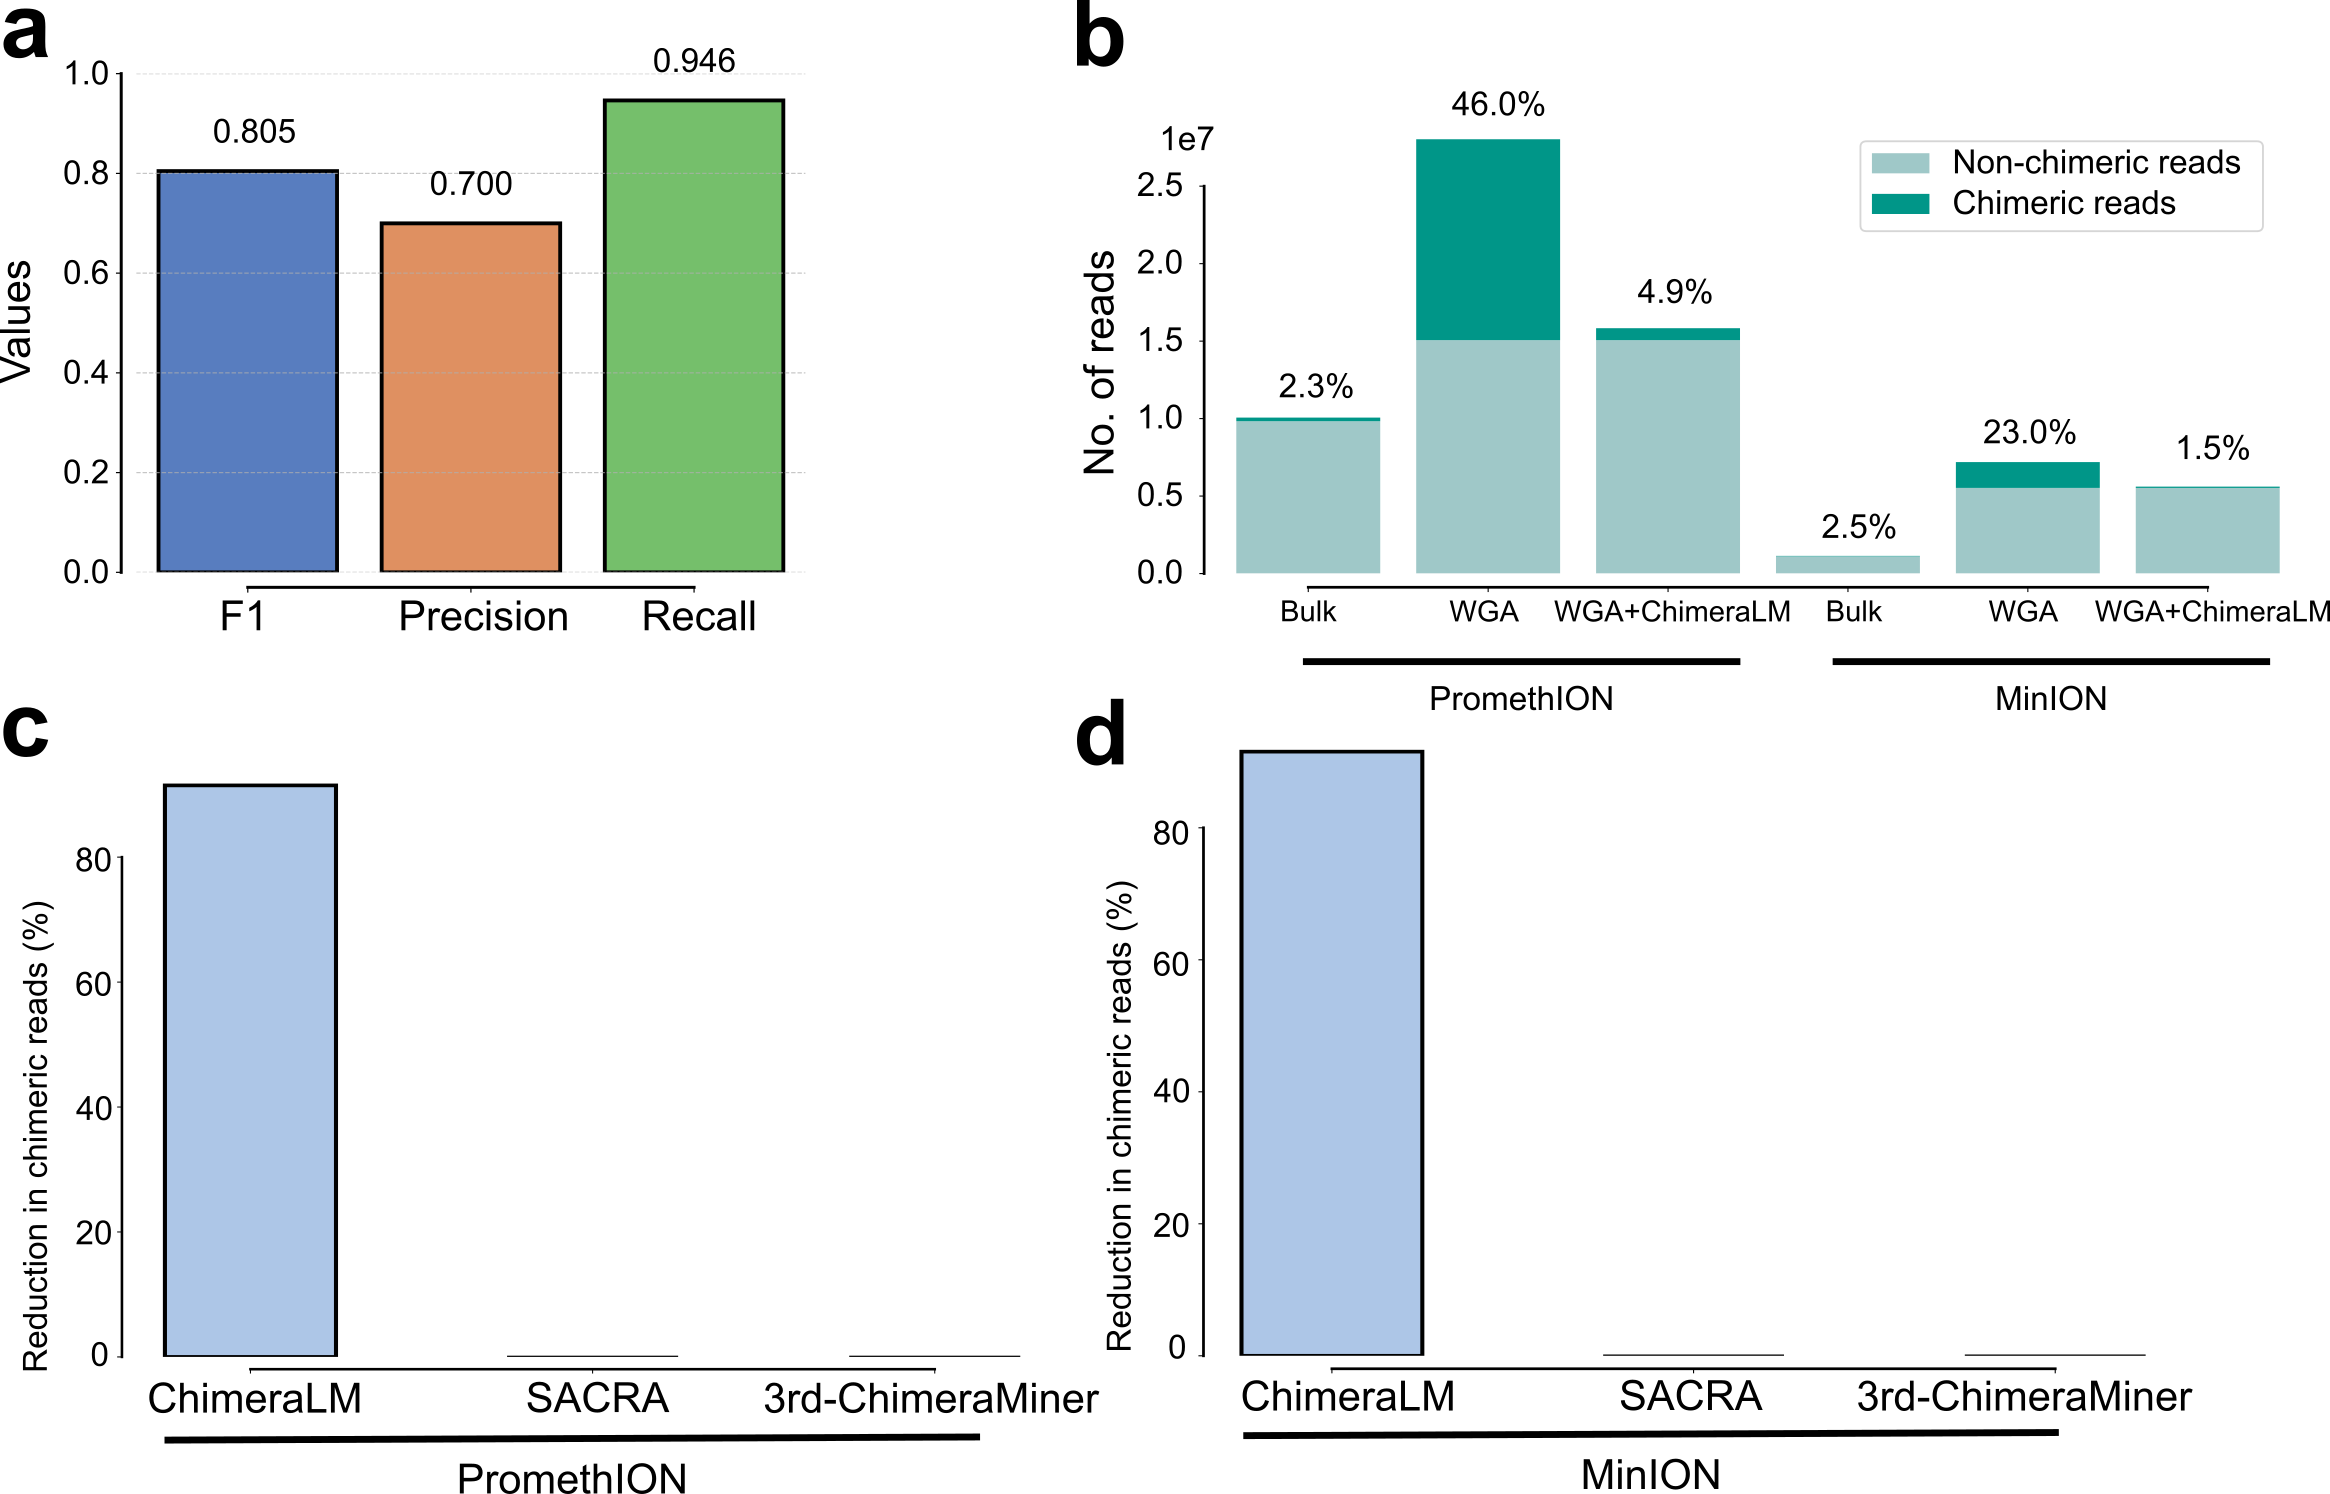
\includegraphics[width=0.95\textwidth]{final_figures/figure2}
	\end{center}
	\caption{Problem and Model}\label{fig:figure2}
\end{figure}


\begin{figure}
	\begin{center}
		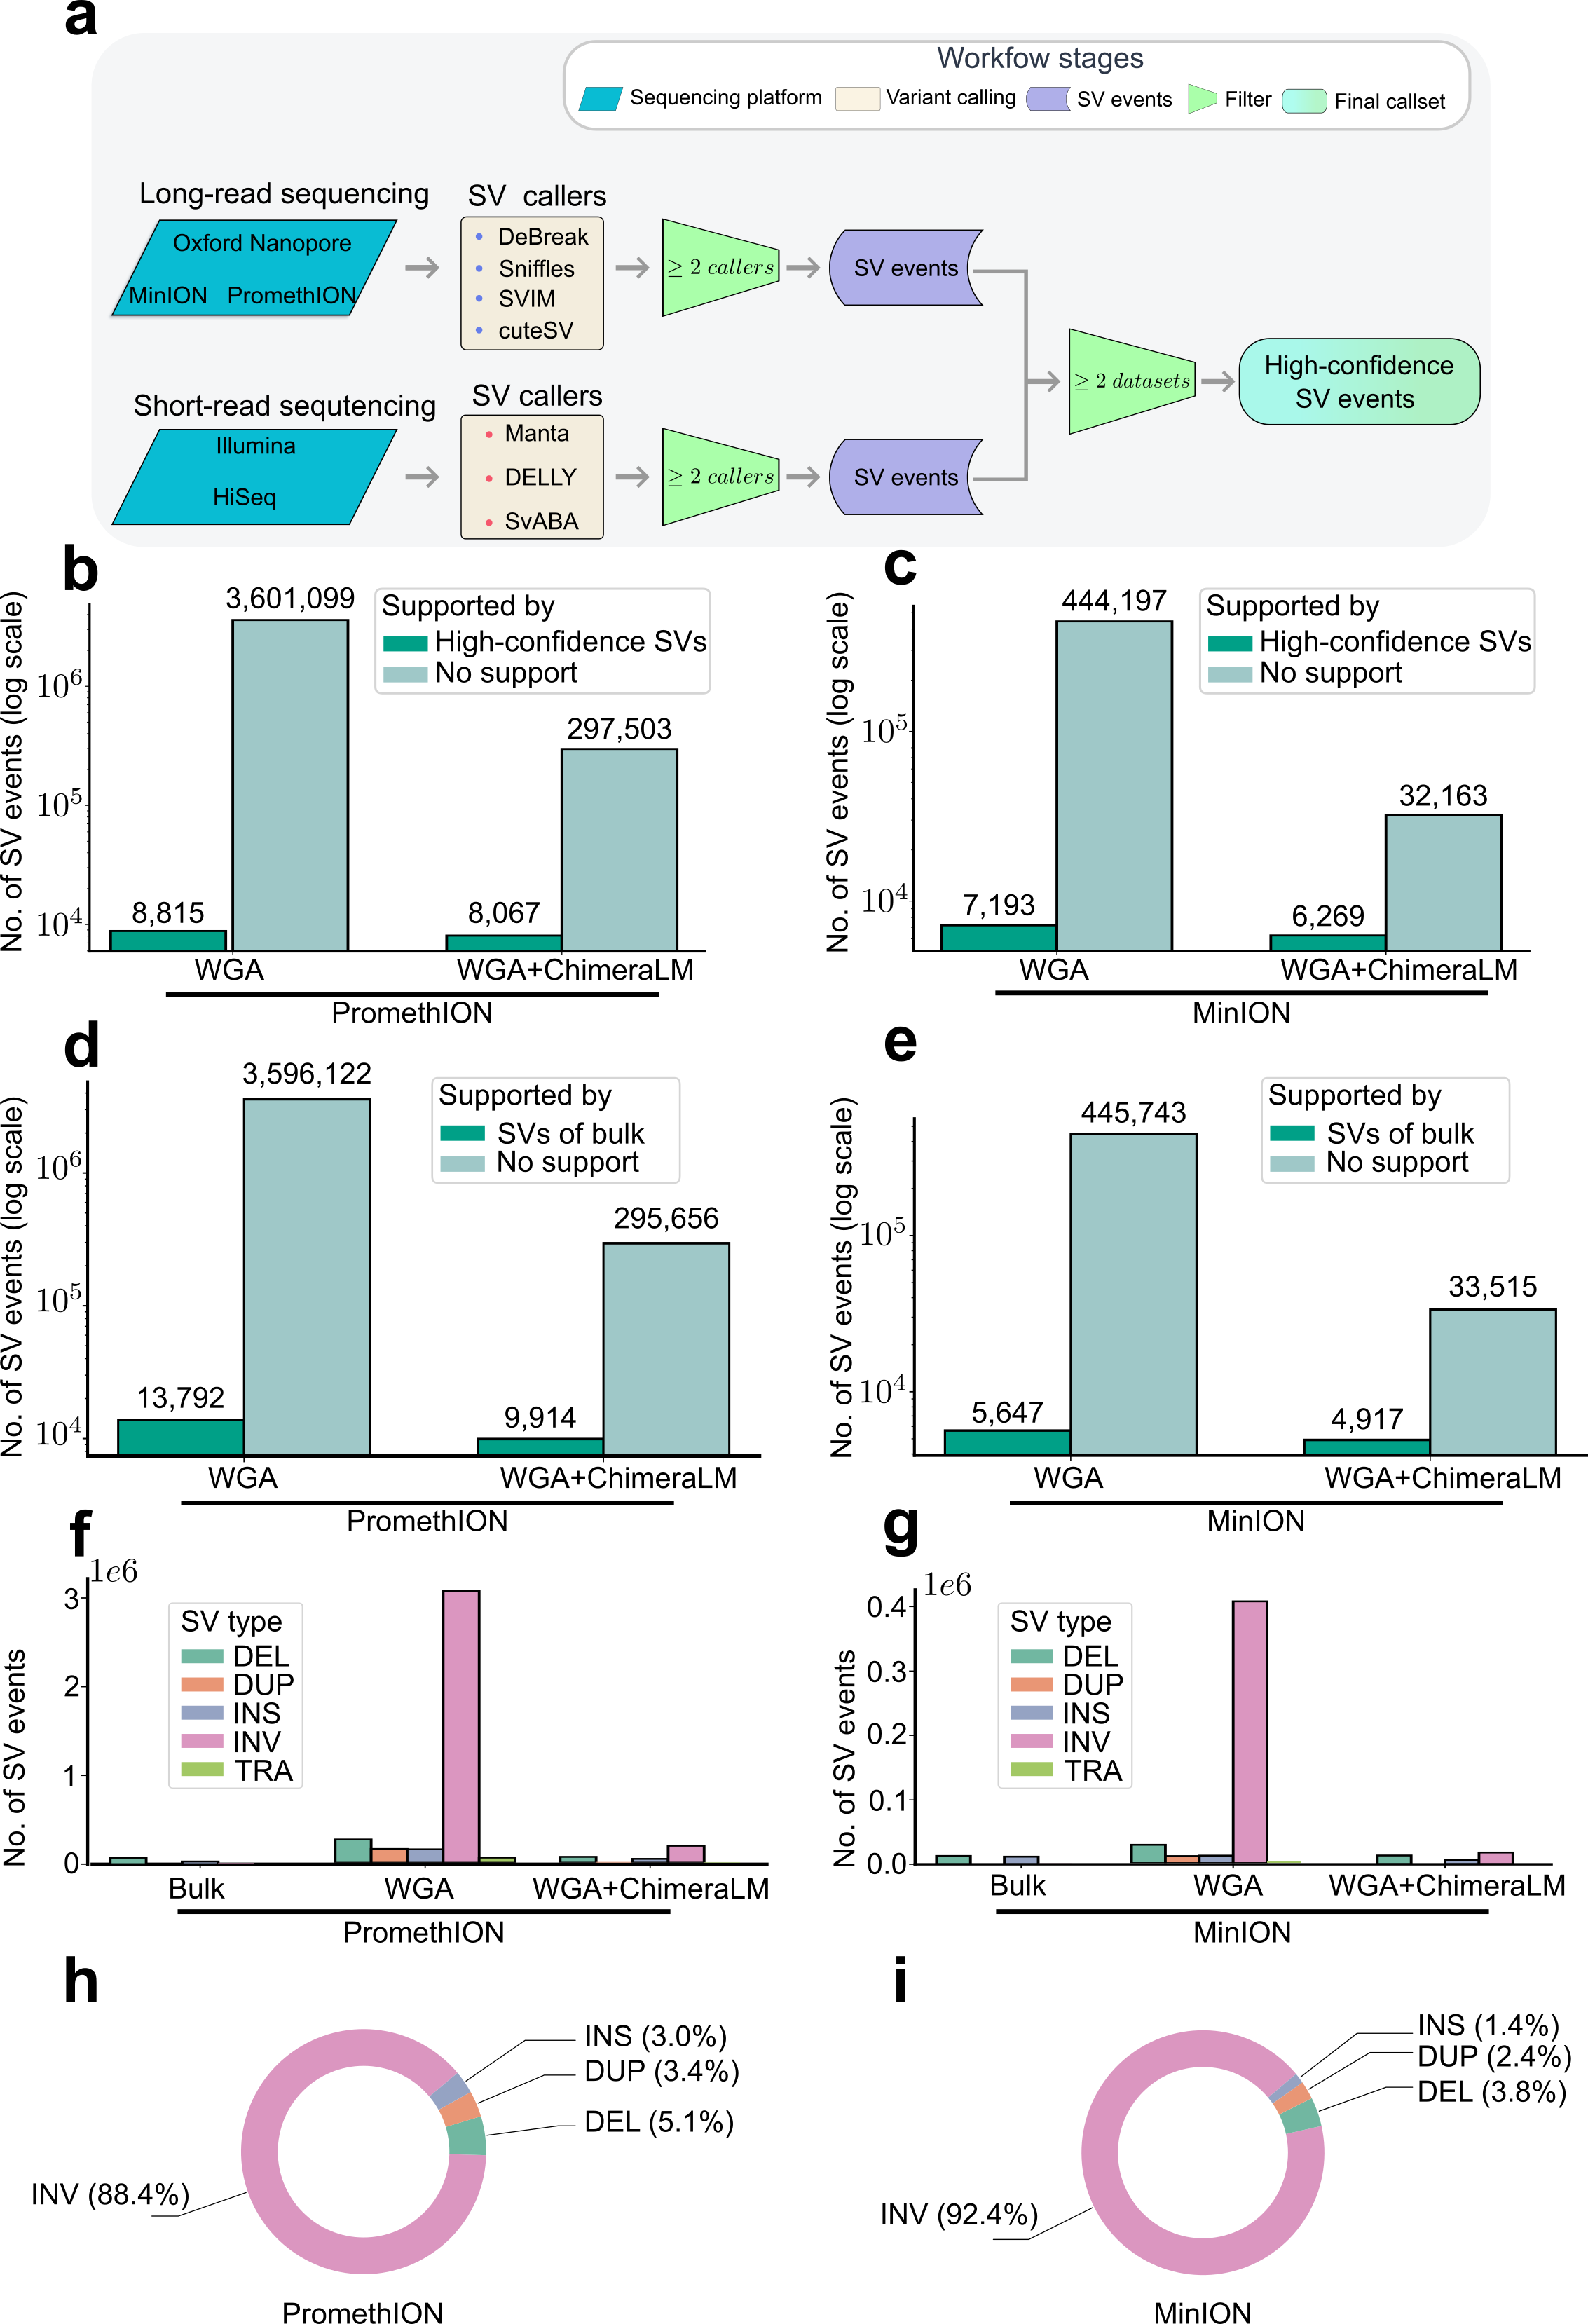
\includegraphics[width=0.95\textwidth]{final_figures/figure3}
	\end{center}
	\caption{Problem and Model}\label{fig:figure3}
\end{figure}

\section*{Methods}\label{sec12}

\subsection*{MDA sequencing}

\subsection*{Train data construction}

\subsection*{Model architecture}

\subsection*{Model training}

\section*{SV evaluation}

\backmatter

\bmhead{Supplementary information}


\begin{figure}
	\begin{center}
		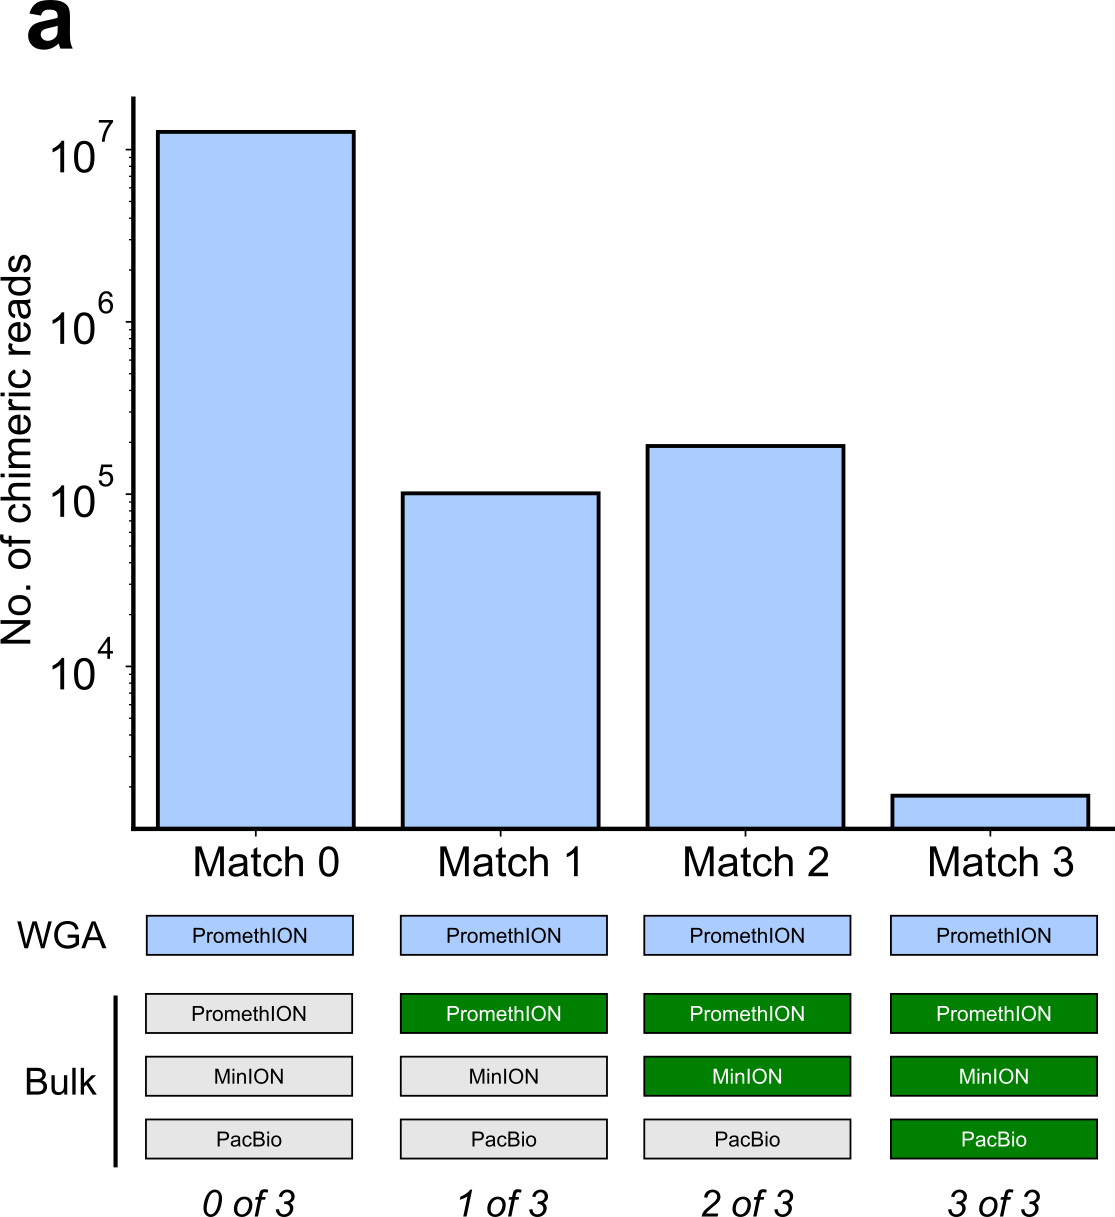
\includegraphics[width=0.8\textwidth]{final_figures/sf1}
	\end{center}
	\caption{Problem and Model}\label{fig:sf1}
\end{figure}


\begin{figure}
	\begin{center}
		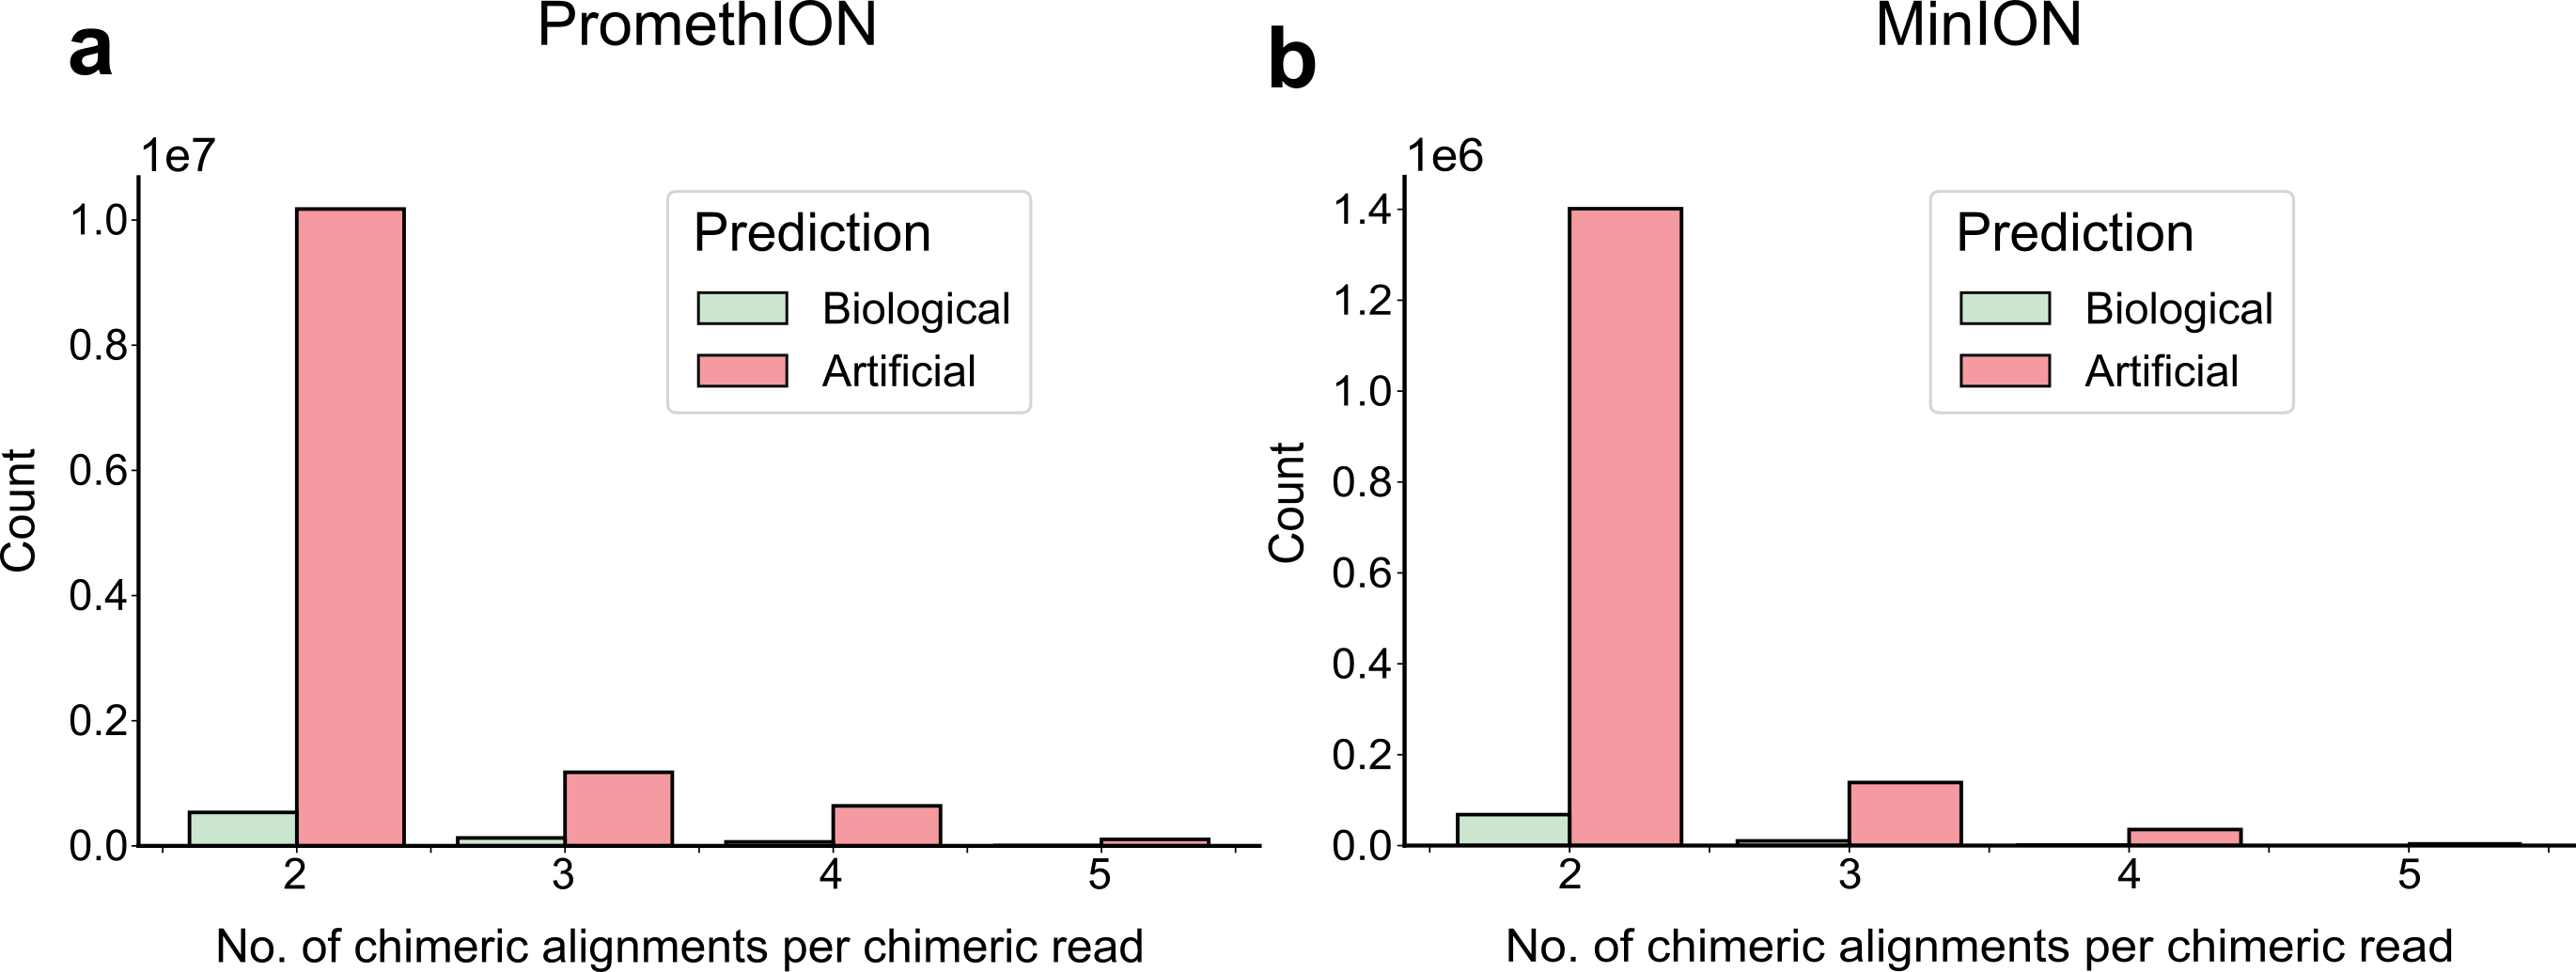
\includegraphics[width=\textwidth]{final_figures/sf2}
	\end{center}
	\caption{Problem and Model}\label{fig:sf2}
\end{figure}

This separation aligns with how many transcript assembly algorithms work:

\begin{enumerate}[leftmargin=*]
	\item First, chains of exons and splice junctions are identified from the data
	\item Then, potential transcripts are derived by traversing the graph in different ways
	\item Finally, relationships between different transcript graphs are established
\end{enumerate}

\bmhead{Acknowledgements}

Acknowledgements are not compulsory. Where included they should be brief. Grant or contribution numbers may be acknowledged.

Please refer to Journal-level guidance for any specific requirements.

\section*{Declarations}

Some journals require declarations to be submitted in a standardised format. Please check the Instructions for Authors of the journal to which you are submitting to see if you need to complete this section. If yes, your manuscript must contain the following sections under the heading `Declarations':

\begin{itemize}
	\item Funding
	\item Conflict of interest/Competing interests (check journal-specific guidelines for which heading to use)
	\item Ethics approval and consent to participate
	\item Consent for publication
	\item Data availability
	\item Materials availability
	\item Code availability
	\item Author contribution
\end{itemize}

\noindent
If any of the sections are not relevant to your manuscript, please include the heading and write `Not applicable' for that section.

\begin{flushleft}%
	Editorial Policies for:

	\bigskip\noindent
	Springer journals and proceedings: \url{https://www.springer.com/gp/editorial-policies}

	\bigskip\noindent
	Nature Portfolio journals: \url{https://www.nature.com/nature-research/editorial-policies}

	\bigskip\noindent
	\textit{Scientific Reports}: \url{https://www.nature.com/srep/journal-policies/editorial-policies}

	\bigskip\noindent
	BMC journals: \url{https://www.biomedcentral.com/getpublished/editorial-policies}
\end{flushleft}

\begin{appendices}

	\printglossaries

	\section{Section title of first appendix}\label{secA1}

	An appendix contains supplementary information that is not an essential part of the text itself but which may be helpful in providing a more comprehensive understanding of the research problem or it is information that is too cumbersome to be included in the body of the paper.

	%%=============================================%%
	%% For submissions to Nature Portfolio Journals %%
	%% please use the heading ``Extended Data''.   %%
	%%=============================================%%

	%%=============================================================%%
	%% Sample for another appendix section			       %%
	%%=============================================================%%

	%% \section{Example of another appendix section}\label{secA2}%
	%% Appendices may be used for helpful, supporting or essential material that would otherwise
	%% clutter, break up or be distracting to the text. Appendices can consist of sections, figures,
	%% tables and equations etc.

\end{appendices}

%%===========================================================================================%%
%% If you are submitting to one of the Nature Portfolio journals, using the eJP submission   %%
%% system, please include the references within the manuscript file itself. You may do this  %%
%% by copying the reference list from your .bbl file, paste it into the main manuscript .tex %%
%% file, and delete the associated \verb+\bibliography+ commands.                            %%
%%===========================================================================================%%

\bibliography{sn-bibliography}% common bib file
%% if required, the content of .bbl file can be included here once bbl is generated
%%\input sn-article.bbl

\end{document}
